
%%*************************************************************************
%%
%% Analysis of Biosignals by Biologically Inspired Algorithms
%% V1.0
%% 2011/05/05
%% by Peter Boraros
%% See:
%% http://www.pborky.sk/contact
%% for current contact information.
%%
%% Desription goes here.
%%
%%
%%*************************************************************************
%% Legal Notice:
%%
%% This code is offered as-is without any warranty either expressed or
%% implied; without even the implied warranty of MERCHANTABILITY or
%% FITNESS FOR A PARTICULAR PURPOSE! 
%% User assumes all risk.
%%
%% This work by Peter Boraros is licensed under a 
%% Creative Commons Attribution-NonCommercial-ShareAlike 3.0 Unported License.
%% http://creativecommons.org/licenses/by-nc-sa/3.0/


\documentclass[a4paper,journal]{IEEEtran}
\ifCLASSOPTIONcompsoc
	\usepackage[nocompress]{cite}
\else
	\usepackage{cite}
\fi

\ifCLASSINFOpdf
	\usepackage[pdftex]{graphicx}
	\graphicspath{{./img/}}
	\DeclareGraphicsExtensions{.pdf}
\else
	\usepackage[dvips]{graphicx}
	\graphicspath{{./img/}}
	\DeclareGraphicsExtensions{.eps}
\fi

\usepackage[cmex10]{amsmath}
\usepackage{amsfonts}
\usepackage{amssymb}
\interdisplaylinepenalty=2500

\usepackage{algorithmic}

\usepackage{array}

\usepackage{mdwmath}
\usepackage{mdwtab}

\usepackage{eqparbox}

\ifCLASSOPTIONcompsoc
	\usepackage[tight,normalsize,sf,SF]{subfigure}
\else
	\usepackage[tight,footnotesize]{subfigure}
\fi

\ifCLASSOPTIONcompsoc
	\usepackage[caption=false,font=normalsize,labelfont=sf,textfont=sf]{subfig}
\else
	\usepackage[caption=false,font=footnotesize]{subfig}
\fi


\usepackage[utf8x]{inputenc}
\usepackage{url}
\usepackage{fixltx2e}
\usepackage{stfloats}
\usepackage{ucs}

% correct bad hyphenation here
\hyphenation{op-tical net-works semi-conduc-tor}

% IEEEtran contains the IEEEeqnarray family of commands that can be used to
% generate multiline equations as well as matrices, tables, etc., of high
% quality.

% stfloats.sty was written by Sigitas Tolusis. This package gives LaTeX2e
% the ability to do double column floats at the bottom of the page as well
% as the top. (e.g., "\begin{figure*}[!b]" is not normally possible in
% LaTeX2e). It also provides a command:
%\fnbelowfloat
% to enable the placement of footnotes below bottom floats (the standard
% LaTeX2e kernel puts them above bottom floats). This is an invasive package
% which rewrites many portions of the LaTeX2e float routines. It may not work
% with other packages that modify the LaTeX2e float routines. The latest
% version and documentation can be obtained at:
% http://www.ctan.org/tex-archive/macros/latex/contrib/sttools/
% Documentation is contained in the stfloats.sty comments as well as in the
% presfull.pdf file. Do not use the stfloats baselinefloat ability as IEEE
% does not allow \baselineskip to stretch. Authors submitting work to the
% IEEE should note that IEEE rarely uses double column equations and
% that authors should try to avoid such use. Do not be tempted to use the
% cuted.sty or midfloat.sty packages (also by Sigitas Tolusis) as IEEE does
% not format its papers in such ways.


\begin{document}
\title{Analysis of biosignals by means of\\ biologically inspired algorithms}

\author{Peter~Boraros% <-this % stops a space
%\IEEEcompsocitemizethanks{
%	\IEEEcompsocthanksitem P. Boraros is with Department of Cybernetics, 
%		Czech Technical University, Prague, Czech Republic.\protect\\
%		E-mail: see http://www.pborky.sk/contact}
}



% The paper headers
\markboth{Peter Boraros, Czech technical university, Faculty of Electrical Engineering,
Prague, Czech Republic}%
{Shell \MakeLowercase{\textit{et al.}}: Bare Demo of IEEEtran.cls for Computer Society Journals}

\IEEEcompsoctitleabstractindextext{%
\begin{abstract}
The aim of this document is to show the usage of biologically inspired algorithms
in analysis of facial electromyography (EMG) and electroencephalography (EEG).
Concretelly, it depicts the process of obtaining data, preprocessing using fast fourier
transform and classifing by means of self-organizing maps (SOM). 
Searching through the parameter space in order to find proper parametrisation of whole
classification process is performed by evolutionary algorithm (EA).
\end{abstract}}

\maketitle
\IEEEdisplaynotcompsoctitleabstractindextext
\IEEEpeerreviewmaketitle


\section{Introduction}
\IEEEPARstart{S}{submission} to this work is to implement methods for analysis 
EMG and EEG signals in order to allow estimation of the subject`s mimics, 
feelings or enable ability to classify the sleep stages and possibly control 
external equipment during specific sleep stage.

\subsection{Signal}
The signal for this research was obtained using device 
\textbf{Nia game controller}, made by 
\textbf{OCZ Techologies}.
It needs no special software driver.
This device provides HID standard interface.
After it is connected, it starts to send 24-bit samples, 
sampled at frequency 4kHz. 
Data represents time series of voltage between two electrodes.
The device has only one balanced channel, thus 
it is not possible to preform complex analysis of neural signals,
however for detection of EMG signal it is sufficient.

Training information is attached during data gathering by human operator.
The raw data from device is saved along with class information from
SW user interface.

Sampling frequency is quite high so the frequency should be reduced to limit
computational complexity. Frequency reduction is performed
by averaging samples. Classification information is reduced by electing
most frequent samples. Reduction rate of the frequency is one of the 
parameters that to be sought.

\subsection{Spectrums}
Raw signal has to be transformed from time domain to frequency domain.
At first it is choped into overlaping slices (windows).
Then fast fourier transform is aplied to each slice. This results in set of 
complex spectral components of same size like time windows.
Phase information should be discarded.

Spectral components are subject to normalisation.
There are several algorithms to choose. Best seems to be 
discrete histogram equlization with scaling the values between [0, 1].
Other possibilities are logistic or range normalisation, that again normalize
values between [0, 1].

Window size, overlap and normalisation algorithm are parameters that to be sought.


\subsection{Self-organizing map}
Self-organising map is method of vector quantisation that can be used to 
cluster analysis. Clusters are represented by best matching units (BMUs)
- vectors that are conected in topological structure. Their value is calculated
by iterative process using training data. Topological neighborhood plays 
also important role and it distincts this method from k-means cluster analysis.
After iterations BMUs should represent real clusters in data.

This unsupervised process can be turned to supervised by adding a classification
information before process.
Class information  could be encoded with 1 of N encoding and appended to the 
spectral vectors. After training it is removed from BMUs and class is 
decoded from 1 of N code as maximal component of appended part.

The spatial 
layout of topological surface has to be checked. It should not contain irregularites, 
the surface should be 'plain' and it should follow the data and the clusters. 
The tolopological error is the criterion to check.

Another criterion is validation/testing error. Traning set is divided into k-folds
and using k-fold crossvalidation the map is trained using k-1 folds and  error 
is determined using the rest fold. This is repeated for each fold. Average error is 
the subject to minimize.
%TODO: link to more detailed descprition


\subsection{Evolutionary algorithm}
The whole process can be parametrised by many parameters. Optimal parametrisation 
is that maximizes correctness e.g. criterion like validation error, resp. correctness.
The other objectives may be e.g. size of window and overlap
should be minimal, computing time should not exceed given boundary, etc.
The parameters can be determined by heuristics upon the whole search space and
is based to prior knowledge of researcher.
Automatic way is to search the search space by search algorithm. This document
describes usage of evolutionary algorithm.
Preferable is to find more solutions that are quite close to optima, instead of 
finding single solution. That allows further heuristics upon the results.

Evolutionary algorithm is inspired by nature and process of evolution...
%TODO: link to proof how and why it works

\begin{figure}[!t]
\centering
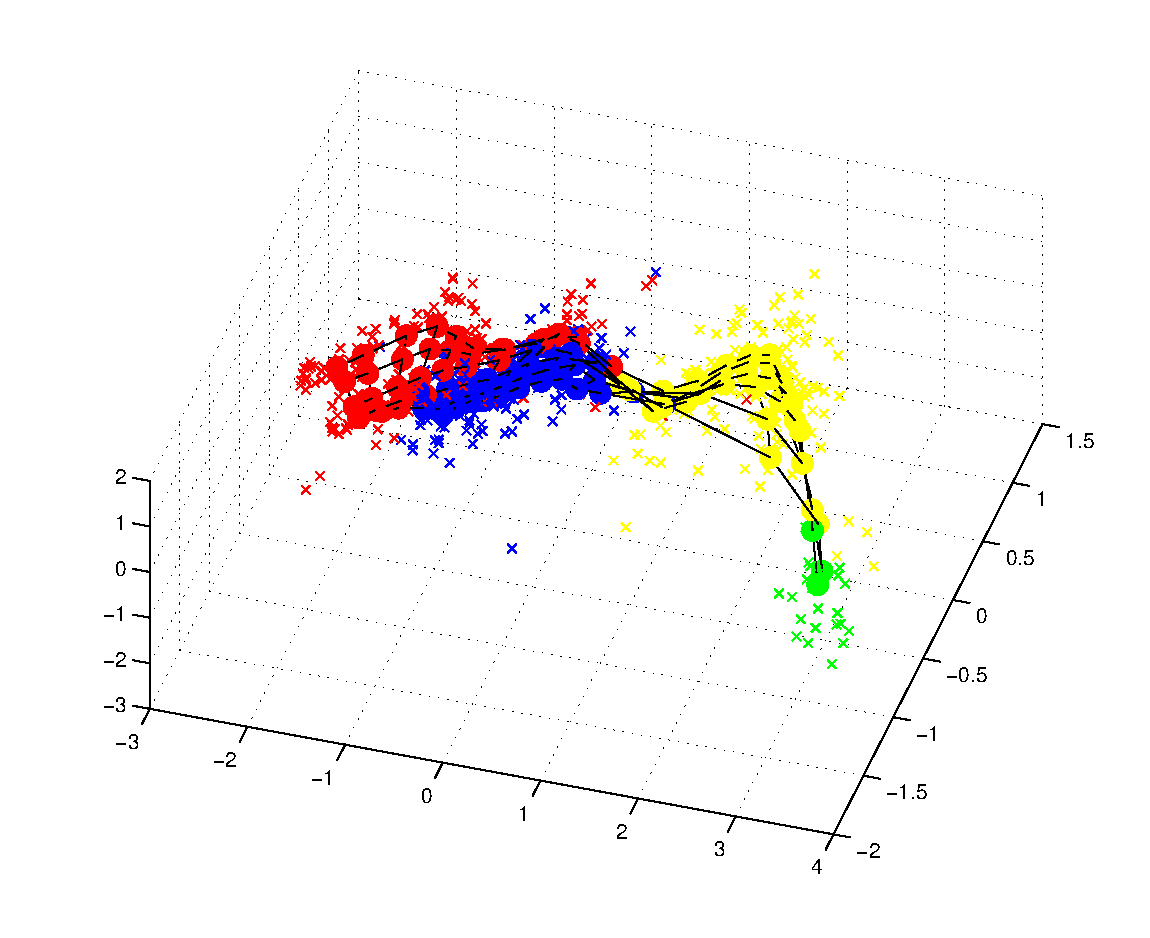
\includegraphics[width=80mm]{som_topol_proj}
% where an .eps filename suffix will be assumed under latex, 
% and a .pdf suffix will be assumed for pdflatex; or what has been declared
% via \DeclareGraphicsExtensions.
\caption{Projection of topology of self-organizing map along with a data}
\label{som_topol_proj}
\end{figure}

\begin{figure}[!t]
\centering
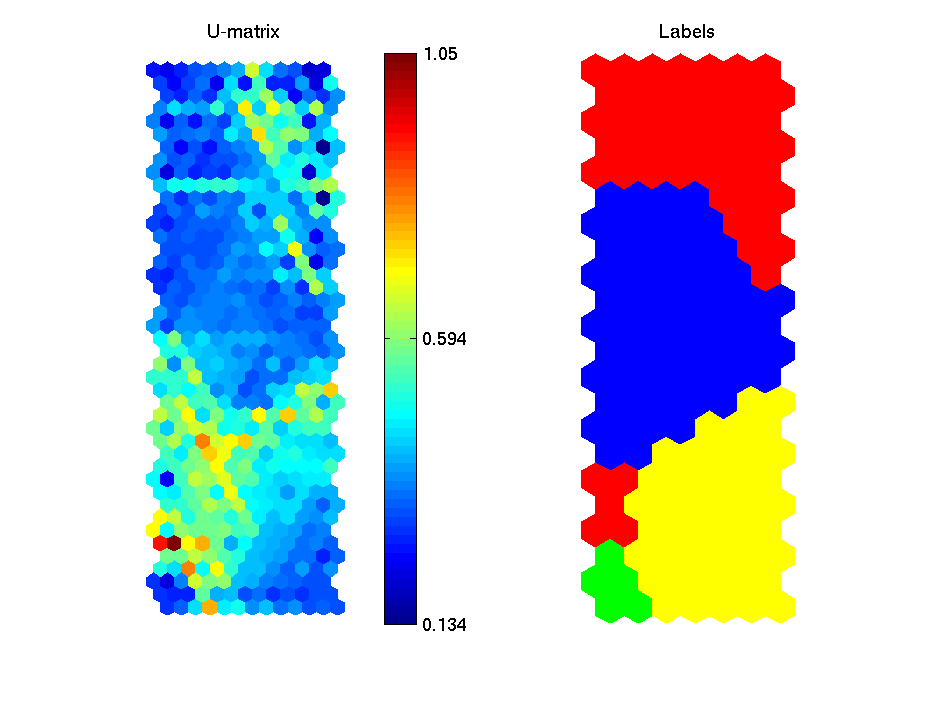
\includegraphics[width=80mm]{som_umat}
% where an .eps filename suffix will be assumed under latex, 
% and a .pdf suffix will be assumed for pdflatex; or what has been declared
% via \DeclareGraphicsExtensions.
\caption{U-matrix and classification of BMUs}
\label{som_umat}
\end{figure}

% An example of a floating figure using the graphicx package.
% Note that \label must occur AFTER (or within) \caption.
% For figures, \caption should occur after the \includegraphics.
% Note that IEEEtran v1.7 and later has special internal code that
% is designed to preserve the operation of \label within \caption
% even when the captionsoff option is in effect. However, because
% of issues like this, it may be the safest practice to put all your
% \label just after \caption rather than within \caption{}.
%
% Reminder: the "draftcls" or "draftclsnofoot", not "draft", class
% option should be used if it is desired that the figures are to be
% displayed while in draft mode.
%

% Note that IEEE typically puts floats only at the top, even when this
% results in a large percentage of a column being occupied by floats.
% However, the Computer Society has been known to put floats at the bottom.


% An example of a double column floating figure using two subfigures.
% (The subfig.sty package must be loaded for this to work.)
% The subfigure \label commands are set within each subfloat command, the
% \label for the overall figure must come after \caption.
% \hfil must be used as a separator to get equal spacing.
% The subfigure.sty package works much the same way, except \subfigure is
% used instead of \subfloat.
%
%\begin{figure*}[!t]
%\centerline{\subfloat[Case I]\includegraphics[width=2.5in]{subfigcase1}%
%\label{fig_first_case}}
%\hfil
%\subfloat[Case II]{\includegraphics[width=2.5in]{subfigcase2}%
%\label{fig_second_case}}}
%\caption{Simulation results}
%\label{fig_sim}
%\end{figure*}
%
% Note that often IEEE papers with subfigures do not employ subfigure
% captions (using the optional argument to \subfloat), but instead will
% reference/describe all of them (a), (b), etc., within the main caption.


% An example of a floating table. Note that, for IEEE style tables, the 
% \caption command should come BEFORE the table. Table text will default to
% \footnotesize as IEEE normally uses this smaller font for tables.
% The \label must come after \caption as always.
%
%\begin{table}[!t]
%% increase table row spacing, adjust to taste
%\renewcommand{\arraystretch}{1.3}
% if using array.sty, it might be a good idea to tweak the value of
% \extrarowheight as needed to properly center the text within the cells
%\caption{An Example of a Table}
%\label{table_example}
%\centering
%% Some packages, such as MDW tools, offer better commands for making tables
%% than the plain LaTeX2e tabular which is used here.
%\begin{tabular}{|c||c|}
%\hline
%One & Two\\
%\hline
%Three & Four\\
%\hline
%\end{tabular}
%\end{table}


% Note that IEEE does not put floats in the very first column - or typically
% anywhere on the first page for that matter. Also, in-text middle ("here")
% positioning is not used. Most IEEE journals use top floats exclusively.
% However, Computer Society journals sometimes do use bottom floats - bear
% this in mind when choosing appropriate optional arguments for the
% figure/table environments.
% Note that, LaTeX2e, unlike IEEE journals, places footnotes above bottom
% floats. This can be corrected via the \fnbelowfloat command of the
% stfloats package.



\section{Conclusion}
The conclusion goes here.





% if have a single appendix:
%\appendix[Proof of the Zonklar Equations]
% or
%\appendix  % for no appendix heading
% do not use \section anymore after \appendix, only \section*
% is possibly needed

% use appendices with more than one appendix
% then use \section to start each appendix
% you must declare a \section before using any
% \subsection or using \label (\appendices by itself
% starts a section numbered zero.)
%


\appendices
\section{Proof of the First Zonklar Equation}
Appendix one text goes here.

% you can choose not to have a title for an appendix
% if you want by leaving the argument blank
\section{}
Appendix two text goes here.


% use section* for acknowledgement
\ifCLASSOPTIONcompsoc
  % The Computer Society usually uses the plural form
  \section*{Acknowledgments}
\else
  % regular IEEE prefers the singular form
  \section*{Acknowledgment}
\fi


The authors would like to thank...


% Can use something like this to put references on a page
% by themselves when using endfloat and the captionsoff option.
\ifCLASSOPTIONcaptionsoff
  \newpage
\fi



% trigger a \newpage just before the given reference
% number - used to balance the columns on the last page
% adjust value as needed - may need to be readjusted if
% the document is modified later
%\IEEEtriggeratref{8}
% The "triggered" command can be changed if desired:
%\IEEEtriggercmd{\enlargethispage{-5in}}

% references section

% can use a bibliography generated by BibTeX as a .bbl file
% BibTeX documentation can be easily obtained at:
% http://www.ctan.org/tex-archive/biblio/bibtex/contrib/doc/
% The IEEEtran BibTeX style support page is at:
% http://www.michaelshell.org/tex/ieeetran/bibtex/
%\bibliographystyle{IEEEtran}
% argument is your BibTeX string definitions and bibliography database(s)
%\bibliography{IEEEabrv,../bib/paper}
%
% <OR> manually copy in the resultant .bbl file
% set second argument of \begin to the number of references
% (used to reserve space for the reference number labels box)
\begin{thebibliography}{1}

\bibitem{IEEEhowto:kopka}
H.~Kopka and P.~W. Daly, \emph{A Guide to \LaTeX}, 3rd~ed.\hskip 1em plus
  0.5em minus 0.4em\relax Harlow, England: Addison-Wesley, 1999.

\end{thebibliography}

% biography section
% 
% If you have an EPS/PDF photo (graphicx package needed) extra braces are
% needed around the contents of the optional argument to biography to prevent
% the LaTeX parser from getting confused when it sees the complicated
% \includegraphics command within an optional argument. (You could create
% your own custom macro containing the \includegraphics command to make things
% simpler here.)
%\begin{biography}[{\includegraphics[width=1in,height=1.25in,clip,keepaspectratio]{mshell}}]{Michael Shell}
% or if you just want to reserve a space for a photo:

\begin{IEEEbiography}{Michael Shell}
Biography text here.
\end{IEEEbiography}

% if you will not have a photo at all:
\begin{IEEEbiographynophoto}{John Doe}
Biography text here.
\end{IEEEbiographynophoto}

% insert where needed to balance the two columns on the last page with
% biographies
%\newpage

\begin{IEEEbiographynophoto}{Jane Doe}
Biography text here.
\end{IEEEbiographynophoto}

% You can push biographies down or up by placing
% a \vfill before or after them. The appropriate
% use of \vfill depends on what kind of text is
% on the last page and whether or not the columns
% are being equalized.

%\vfill

% Can be used to pull up biographies so that the bottom of the last one
% is flush with the other column.
%\enlargethispage{-5in}



% that's all folks
\end{document}


